\documentclass[a4paper,10pt]{report}

\usepackage{graphicx}
\usepackage{color}

\usepackage{caption}
\usepackage{subcaption}

\usepackage[portuguese]{babel}
\usepackage[utf8]{inputenc}
\usepackage[T1]{fontenc}

\usepackage{geometry}
\geometry{a4paper}
\usepackage[parfill]{parskip}

\usepackage{changepage}

\usepackage{amsmath}

\usepackage{fancyhdr}

\usepackage{nopageno}

\graphicspath{{./imagens/}}

\usepackage{url}

\usepackage{verbatim}
\usepackage{fancyvrb}
\usepackage{listings}

\usepackage[colorlinks=true,linkcolor=blue,citecolor=blue]{hyperref}

\usepackage{listings}
\renewcommand{\lstlistingname}{Código}
\usepackage{color}
\definecolor{grey}{rgb}{0.9,0.9,0.9}
\definecolor{greyD}{rgb}{0.5,0.5,0.5}

\lstnewenvironment{code}[1][]%
{
   \noindent
   \lstset{
  language=C,
  float=htpb,
  backgroundcolor=\color{grey},
  basicstyle=\scriptsize,
  numbers=left,
  numbersep=5pt,
  numberstyle=\tiny\color{greyD},
  breaklines=true,
  frame=single,
  #1}
}
{}

\begin{document}

\begin{titlepage}
\begin{center}

\begin{flushleft}

\includegraphics[height=3.00cm]{EENG.jpg}\\
\end{flushleft}

\vspace{1.5cm}

\Large{\textbf{LEI --- Licenciatura de Engenharia Informática}}\\
\vspace{1cm}
\Large{\textbf{Processamento de Linguagens}}\\

\vspace{1cm}

\Huge{\textbf{Compilador de uma LPIS}} \\

\vspace{2cm}

\Large{\textbf{Orlando Costa -  a67705, Paulo Araujo - a58925, Rui Oliveira - a67661}}\\
\begin{figure}[h]
\centering
\begin{subfigure}{.3\textwidth}
  \centering
  
\includegraphics[width=\textwidth]{Orlando.jpg}
\end{subfigure}
\begin{subfigure}{.3\textwidth}
  \centering
  
\includegraphics[width=\textwidth]{Paulo.jpg}
\end{subfigure}
\begin{subfigure}{.3\textwidth}
  \centering
  
\includegraphics[width=\textwidth]{Oliveira.jpg}
\end{subfigure}
\end{figure}

\vspace{1.5cm}
Braga, 7 de Junho de 2015

\end{center}

\end{titlepage}


\begin{abstract}
Este relatório descreve a resolução de um conjunto de exercícios propostos, que consistem no desenvolvimento de programas na linguagem C com o auxílio de geradores de filtros de texto, como o Flex. Para cada problema é realizada uma breve análise sobre o trabalho efetuado, as decisões que lideraram o seu desenvolvimento e as estruturas implementadas, assim como uma explicação do seu funcionamento. 

Os problemas resolvidos consistem no desenvolvimento de filtros de texto que:
\begin{itemize}
\item processa um ficheiro XML com descrições de fotografias e gerar um álbum HTML.
\item processa de um ficheiro XML anotado com tags Enamex e gera páginas HTML apresentando as "pessoas", "países", "cidades" e organizações nele identificadas. 
\item processa vários ficheiros de texto, compostos por letras de canções, e gera documentos em LATEX para cada uma delas.
\end{itemize}
Para cada problema é apresentado o código em linguagem C e as expressões regulares desenvolvidas, sendo estes suportados por exemplos e devidos resultados.
\end{abstract}
%----------------------------------------------------------------------
%\newpage
%\phantom{placeholder} % doesn't appear on page
%\thispagestyle{empty} % if want no header/footer
%----------------------------------------------------------------------
\tableofcontents
%\phantom{placeholder} % doesn't appear on page
\thispagestyle{empty} % if want no header/footer
%----------------------------------------------------------------------
%\newpage
%\phantom{placeholder} % doesn't appear on page
%\thispagestyle{empty} % if want no header/footer
%----------------------------------------------------------------------
%\pagestyle{fancy}
%\setlength{\headheight}{15.2pt}
%\fancyhf{} % apagar as configurações actuais
%\fancyfoot[LE,RO]{\thepage}
%\fancyhead[LE,RO]{PL - Trabalho Pratico 1 --- Araujo P., Belo O., Oliveira R.}
%\page{setcounter}{0}
%----------------------------------------------------------------------

\chapter{Introdução}
\label{cap:intro}
O presente projeto enquandra-se na unidade curricular de Processamento de Linguagnes do curso de  Licenciatura em Engenharia Informática da Universidade do Minho.
O projeto pretende aumentar as capacidades com as expressões regulares, desenvolvendo processadores de linguagens regulares utilizando o gerador de filtros de texto Flex.
Para isso foram selecionados 3 exercícios dentro de um grupo de 8 exercícios, são eles: \emph{2.1 Museu da Pessoa — tratamento de fotografias},
\emph{2.2 Processamento de Entidades Nomeadas (Enamex)} e \emph{2.5 Processamento de ficheiros com Canções}.

\chapter{Museu da Pessoa — tratamento de fotografias}
\label{cap:museu}
Neste problema é pretendido que, a partir de um ficheiro \emph{XML}, seja criado um filtro de texto capaz de interpretar informação relativa às entrevistas feitas para construção o Museu da Pessoa. Com toda essa informação, deverá ser criado um álbum em \emph{HTML} possuidor de um índice, ordenado alfabeticamente, contendo todos os nomes de pessoas presentes no álbum. Além disso, cada elemento do índice deverá estar referenciado para a página que contém todas as fotos da respetiva pessoa. Relativamente às fotos, essas deverão estar ordenadas cronologicamente e a descrição da foto deverá ser o seu título/cabeçalho.

\section{Analise e Especificação}
\label{seq:museu-ana}
Após a análise do que é pedido no enunciado e de alguns dos \emph{Datasets}, foi possível verificar qual a informação essencial a retirar do ficheiro \emph{XML}. Além disso, como não é regra que as fotos e pessoas presentes no ficheiro \emph{XML} estejam já na ordem pretendida, será necessário que toda a informação seja armazenada em estruturas de dados. O nome do ficheiro \emph{HTML} resultante, poderá ser dado como argumento e caso não seja, por omissão será \emph{AlbumGerado.html}. Além deste ficheiro, serão gerados tantos ficheiros \emph{HTML} quantas as pessoas presentes no álbum. Esses ficheiros serão denominados numericamente (1.html,2.html,...) à medida que novos nomes são encontrados. Os ficheiros anteriormente referidos apenas serão gerados no final da leitura e filtragem de ficheiro \emph{XML}.


\section{Implementação}
\label{seq:museu-imp}
\subsection{Estrutura de dados}
\label{seq:museu-est}
De forma a dar seguimento ao que foi especificado na secção \ref{seq:museu-ana}, foi necessária a criação de uma estrutura de dados que sirva de suporte aos dados recolhidos. Sendo assim, optamos por criar uma estrutura denominada \verb!photo_node! que terá o formato de uma árvore binária e servirá para armazenar toda a informação relativa a cada descrição de fotos encontrada no ficheiro \emph{XML}. Nesta estrutura serão guardados o nome do ficheiro que contém a foto, a data e o local em que esta foi tirada, a sua descrição e o nome das pessoas nela presentes. A inserção de fotos nesta árvore será ordenada relativamente à sua data.
Além desta estrutura, também criamos outra, denominada \verb!person_node!, com o objetivo que esta guarde toda a informação acerca das pessoas presentes no álbum. Esta estrutura tem o formato de uma lista ligada e guardará informação como o nome da pessoa, assim como o nome do ficheiro da sua página \emph{HTML} e terá ainda um apontador para uma estrutura \verb!photo_node! em que será armazenada toda a informação relacionada com as suas fotos. Finalmente, criamos uma estrutura \verb!Album! que apenas conterá um apontador para uma estrutura \verb!person_node!, onde estará a informação relativa às pessoas nele presente, e um contador que servirá para contar o número de pessoas presentes no álbum. O contador servirá de auxílio na criação dás páginas \emph{HTML} numeradas referidas na secção \ref{seq:museu-ana}.

\subsection{Filtro de Texto}
\label{seq:museu-filtro}
Um dos objetivos deste trabalho prático é a utilização de geradores de filtro de texto, como o \emph{Flex}. Sendo assim, foi criado um ficheiro Flex que permite encontrar determinados padrões de expressões regulares e executar uma determinada ação para cada uma delas.

No ficheiro referido, podemos encontrar algumas instruções em \verb!linguagem C! como a inclusão de ficheiros de cabeçalhos ( headers, .h) e a declaração de variáveis.
De seguida, são definidas as expressões regulares e as respetivas ações que se pretendem realizar no caso da identificação positiva do referido padrão:

\verb!\<foto[ \t]+[a-zA-Z]+=\".*\"!
A partir da análise do ficheiro \emph{XML} exemplificado no enunciado, foi possível verificar que a descrição de uma foto começa com o nome do ficheiro que a contem da seguinte forma: \verb!<foto ficheiro="ficheiro.jpg">!. Sendo assim, quando este padrão é encontrado, é inicializado um \verb!photo_node! com o nome encontrado entre as aspas. O nome é obtido retirando da expressão apenas o que se encontra à frente da primeira ocorrência de aspas e atrás da ocorrência seguinte.

\verb!\<quando[ \t]+[a-zA-Z]+=\"[0-9]{4}(.|-)[0-9]{2}(.|-)[0-9]{2}!
De seguida pretendemos encontrar a data em que a foto foi tirada. A partir do exemplo do enunciado, verificamos que a data é descrita da seguinte forma: \verb!<quando data="1961-01-15"/>!. Sendo assim, pretendemos encontrar todas as expressões no formato referido, com a possibilidade que a data esteja separada por pontos em vez de traços. A obtenção da data faz-se retirando apenas o que se encontra à frente da primeira ocorrência de aspas.

\verb!\<quem>[ \t\na-zA-ZÀ-û,\"0-9;:]+!
Um padrão essencial a encontrar é o nome das pessoas presentes na foto. Esses nomes devem estar descritos da seguinte forma: \\
\verb!<quem>Ana de Lourdes de Oliveira Chamine; Antonio Oliveira Machado</quem>!\\
Nesta fase, optamos por não separar ainda os nomes por tokens porque será mais útil fazê-lo apenas quando a descrição da foto estiver completa. Sendo assim, apenas retiramos tudo o que esteja entre \verb!'>'! e \verb!'<'! e adicionamos à estrutura que contem a descrição da foto.

\verb!\<onde>[ \t\n0-9a-zA-ZÀ-û.,;:\"]+<!
Continuando com a análise do exemplo do enunciado, verificamos que uma foto pode ter descrito o local em que esta foi tirada:\\
\verb!<onde>Casa Machado, Afurada, Vila Nova de Gaia</onde>!\\
Ora, quando este padrão é encontrado, só é necessário guardar o que está entre \verb!'>'! e \verb!'<'!, assim como no caso anterior.

\verb!\<facto>[ \t\n0-9a-zA-ZÀ-û.,;:\"]+<!
Finalmente, o último campo necessário para a descrição da foto é o facto que esta representa: \verb!<facto> Os noivos cortam o bolo de casamento</facto>!. O que é essencial retirar neste caso é o mesmo que nos casos anteriores, ou seja, apenas o que se encontra entre \verb!'>'! e \verb!'<'!.

\verb!\<\/foto>!
Sempre que é encontrado o padrão que finaliza a descrição de uma foto, \verb!</foto>!, é necessário adicionar o \verb!photo_node! criado a todos os respetivos \verb!person_node! das pessoas que se encontram na descrição da foto. É nesta fase que os nomes das pessoas presentes na foto é separado e identificado. Finalmente adiciona-se a descrição da foto a todas as pessoas nela presente.

\verb!.|\n!
Este padrão apenas é utilizado para indicar que sempre que é encontrado qualquer outro \verb!byte! ou \verb!\n!, deve ser ignorado.

\subsection{Funcionamento}
\label{seq:museu-func}
Antes do filtro de texto ser aplicado ao ficheiro \emph{XML} é invocada a função \verb!init! que inicializa uma variável \verb!static Album!. Inicializada esta variável, é possível aplicar o filtro de texto.
À medida que a informação do ficheiro \emph{XML} é filtrada, são invocadas funções que tratam e guardam na estrutura a informação recolhida.
Sempre que é encontrada uma expressão que defina o início de uma descrição de uma foto, a informação relativa ao nome da foto é recolhida e é invocada a função \verb!initPhoto! que trata de alocar o espaço necessário para a informação que virá a ser recolhida posteriormente. Do mesmo modo, sempre que é encontrada uma expressão que identifique a data, a localização, a descrição ou as pessoas presentes na foto, são invocadas funções capazes de tratar e armazenar essa informação. As funções referidas são \verb!setDate, setLoc, setFact e setWho!, respetivamente. Sempre que não seja possível identificar uma destas características anteriores, estas ficam com os seus valores por defeito, ou seja, caso uma foto não tenha a tag \verb!<quem>!, o seu campo correspondente na estrutura ficará preenchido com \verb!"Desconhecidos"!. Finalmente, quando é encontrada a expressão que define o final da descrição de uma foto, é invocada a função que trata de inserir a informação da nova foto na estrutura \verb!Album!.
Depois de tratada toda a informação, são invocadas funções auxiliares que criam e preenchem o(s) ficheiro(s) \emph{HTML} necessários.

\section{Testes realizados}
\label{seq:museu-test}
Estão documentados neste secção 3 testes realizados ao autómato, utilizando como input os ficheiros que se encontram em anexo: \ref{seq:anex-museu-test-in01}, \ref{seq:anex-museu-test-in02}, \ref{seq:anex-museu-test-in03} e \ref{seq:anex-museu-test-in04}.

\subsubsection{Teste nº 1}

Neste teste podemos verificar que apenas existe uma página criada devida à presença de apenas uma pessoa nas fotos.

\subsubsection{Teste nº 2}

Neste teste podemos verificar que as fotos não contêm descrição, visto que o ficheiro XML não contem o campo "<facto>".

\subsubsection{Teste nº 3}

Neste teste podemos verificar que um dos items do indice encontra-se incompleta, por não ser possível a leitura de um caracter.

\subsubsection{Teste nº 4}

Teste exemplificado no enunciado. O nome das pessoas presentes na foto encontram-se separados por ":", pode-se verificar que ambas as páginas respetivas contêm as fotos em comum.


Possíveis exemplos de aplicação deste filtro de texto:
\begin{itemize}
\item\verb!cat\ <inputFile>\ |\ ./play\ <output1.html>\ !
\item\verb!cat\ <inputFile>\ |\ ./play\ !
\end{itemize}
\chapter{Processamento de Entidades Nomeadas}
\label{cap:enamex}

Entidades nomeadas são "elementos atómicos em texto" pertencentes a categorias predefinidas tais como nomes de pessoas, organizações, localizações, quantidades, etc. Assim, Processamento de Entidades Nomeadas(PEN) é a tarefa de identificar estas entidades.
Embora as categorias das entidades nomeadas serem predefinidas, existem várias opiniões sobre que categorias deve ser consideradas entidades nomeadas e quão abrangentes estas categorias devem ser. Por convenção, tags \emph{"ENAMEX"} são utilizadas para nomes, tags \emph{"NUMEX"} são utilizadas para entidades numéricas, e tags \emph{"TIMEX"} são utilizadas para entidades temporais.

Neste exercício iremos apenas processar entidades com a tag \emph{"ENAMEX"}, na forma:
\begin{itemize}
\item\verb!<ENAMEX TYPE="PERSON">Francisco de Vilela Barbosa</ENAMEX>!\\(Pessoa)
\item\verb!<ENAMEX TYPE="LOCATION" SUBTYPE="COUNTRY">Portugal</ENAMEX>!\\ (Localização, País)
\item\verb!<ENAMEX TYPE="LOCATION" SUBTYPE="CITY">Rio de Janeiro</ENAMEX>!\\  (Localização, Cidade)
\item\verb!<ENAMEX TYPE="ORGANIZATION">Universidade do Minho</ENAMEX>!\\(Organização)
\end{itemize}

Como exercício extra iremos também abordar as entidades na forma:
\begin{itemize}
\item\verb!<ENAMEX TYPE="LOCATION"> Santo Novo </ENAMEX>!\\(Localização não específica)
\end{itemize}
Todas as outras tags irão ser ignoradas.

O processamento de entidades nomeadas, apesar de ser aparentemente uma tarefa simples, enfrenta um dado numero de desafios. As entidades podem tornar-se difíceis de encontrar, e uma vez encontradas, difíceis de classificar. Localizações e nomes de pessoas podem ser as mesmas, e seguir estilos similares de formatação.

\section{Analise e Especificação}
\label{seq:enamex-ana}

Uma breve leitura do problema permite-nos entender algumas das funcionalidades necessárias, sendo estas definidas como:
\begin{itemize}
\item Necessidade de ordenação e não repetição na listagem de pessoas(alínea a): \\
	\begin{itemize}
	\item A alínea A do problema requer a listagem de todas as pessoas identificadas, sem repetições. Este informação refere-se então às tags do tipo:\\
	\verb!<ENAMEX TYPE="PERSON">...</ENAMEX>!.\\
	Por forma a armazenar e ordenar adequadamente toda a informação acerca das Pessoas, é necessária a utilização de uma estrutura capaz de suportar esta informação. 
	\end{itemize}
	
\item Listar os países e cidades marcadas (alínea b): \\
	\begin{itemize}
	\item Apesar de não estar especificado no enunciado, o grupo propôs uma implementação na qual seria possível associar cidades a certos países. Compreendemos que este tipo de implementação, para grande parte dos casos, não é viável e pode tornar a informação apresentada incoerente. No entanto, no intuito de aprender e aumentar o desafio proposto, decidimos que cidades mencionadas após países e antes de pontos finais pertenciam a esses países. Esta informação é também armazenada na estrutura implementada.
	\end{itemize}
\item Listar as organizações (alínea c): \\
	\begin{itemize}
	\item Similarmente à alínea A, a alínea C requer a listagem de todas as organizações identificadas. Esta informação refere-se então às tags do tipo: \\
	\verb! <ENAMEX TYPE="ORGANIZATION">...</ENAMEX>! \\
	E está implementada de forma similar à listagem de pessoas.
	\end{itemize}
\item Apresentar os resultados em formato HTML: \\
	\begin{itemize}
	\item Por forma a visualizar facilmente os resultados do processamento do texto, estes são apresentados em formato HTML através da implementação de funções capazes de transformar a informação contida nas estruturas em documentos de texto com o formato requerido.
	\end{itemize}
\end{itemize}

\section{Implementação}
\label{seq:enamex-imp}
\subsection{Estrutura de dados}
\label{seq:enamex-est}
Com o intuito de cumprir todos os requisitos estruturais definidos anteriormente, foi desenvolvida uma estrutura de dados única capaz de armazenar todos os dados necessários. Assim, escolhemos implementar uma árvore binária de procura, na qual os nodos possuem a informação a guardar sobre a forma de array de caracteres. A escolha desta estrutura facilita a ordenação alfabética dos diversos nomes que possamos processar, e é de implementação relativamente simples. Creemos ser superior a outras estruturas tais como listas ligadas cuja implementação, apesar de mais simples, torna-se mais complexa quando é necessária a ordenação dos seus elementos (O(N)) e a tabelas de hash cuja implementação é mais complexa, sendo que para elevadas quantidades de dados possuem ainda a necessidade de reHashing e garbage colection. 

<-tree.png-> ???

Para casos em que apenas é necessário o armazenamento da entidade, sem qualquer tipo de associação, uma árvore com dois apontadores (esquerda e direita) e com a capacidade de armazenar a informação (array de caracteres) bastaria para abordar todos os casos. No entanto, de forma a armazenar a possível associação entre os países e as suas cidades, modificamos a árvore previamente referida, e adicionamos-lhe um apontador extra, que poderá ser visto como o apontador para a raiz de uma nova árvore, constituída por todas as cidades que pertencem a um dado país. Como curiosidade, adicionamos também um inteiro em cada nodo que servirá como contador para todas as ocorrências de um dado elemento. Todo o código referente a esta estrutura encontra-se implementado no ficheiros "tree.c" e "tree.h" e pode ser consultado em anexo.

\subsection{Filtro de Texto}
\label{seq:enamex-filtro}

De forma a processar as tags pertencentes a pessoas/organizações, foram criadas expressões regulares capazes de identificar essas tags.
Assim, foram implementadas as seguintes expressões regulares para pessoas/organizações, assim como abreviaturas que facilitam a sua leitura e compreensão:

\begin{itemize}
\item pessoas: \verb! {enamex}{person}{pal}{eclose}! 
\item organizações:\verb!{enamex}{org}{pal}{eclose}!
\item localizações gerais:\verb! {enamex}{loc}{pal}{eclose}!
\item cidades: \verb!{enamex}{loc}{subcity}{pal}{eclose}!
\end{itemize}

sendo que as abreviaturas mencionadas correspondem a:

\begin{itemize}
\item Palavra \\
	\verb!    {pal} [a-zA-Z0-9Ç-ÑÀ-û ]+!
\item Tag Enamex \\
	\verb!    {enamex} \<[ \t]*(?i:enamex)[ \t]+(?i:type)=!
\item Tag de fecho \\
	\verb!    {eclose} \<[ \t]*\/(?i:enamex)[ \t]*\>!
\item Elemento "Organization"\\
	\verb!    {org} \"[ \t]*(?i:organization)[ \t]*\"[ \t]*\>!
\item Elemento "Person"\\
	\verb!    {person} \"[ \t]*(?i:person)[ \t]*\"[ \t]*\>!
\end{itemize}


De notar a capacidade das expressões regulares identificarem tags definidas tanto em letra maiuscula como minuscula, sendo também tolerantes à quantidade de espaços ou tabs presentes entre elementos destas.
De forma a implementar a capacidade de associar cidades a um dado país, foram utilizados "operadores de contexto", de forma a que caso seja detectado uma tag correspondente a um país, o analisador entre no contexto não exclusivo (\%s)country, e associa as seguintes tags correspondentes a cidades ao país em causa. Caso seja detetado um ponto final, o analisador lexico abandona esse contexto e continua a processar em contexto geral. 

\textbf{Nota}: Esta foi uma funcionalidade assumida, pelo que poderá nem sempre ter sucesso e fazer as corretas associações.

Assim as expressões regulares correspondentes a localizações/países/cidades foram definidas na forma:

\begin{itemize}
\item paises: \\
	\verb!    {enamex}{loc}{subcountry}{pal}{eclose}!
\item ponto final no contexto "country":\\
	\verb!    <country>!
\item cidades no contexto "country":\\
	\verb!    <country>{enamex}{loc}{subcity}{pal}{eclose}!
\end{itemize}

sendo que as abreviaturas mencionadas correspondem a:

\begin{itemize}
\item Elemento "Country"\\
	 \verb!    {subcountry}  (?i:subtype)=\"[ \t]*(?i:country)[ \t]*\"[ \t]*\>!
\item Elemento "City"\\
	 \verb!    {subcity} (?i:subtype)=\"[ \t]*(?i:city)[ \t]*\"[ \t]*\>!
     
\end{itemize}

Estas expressões devem encontrar-se no topo de todas as outras, devido à precedência que possuem sobre elas.

\subsection{Funcionamento}
\label{seq:enamex-func}

No cabeçalho do ficheiro flex são declarados todos os apontadores referentes às estruturas onde irá ser armazenada a informação. Existe um apontador para cada tipo de estrutura, nomeadamente: pessoas, paises, cidades, organizações e outras localizações. São também declarados dois apontadores para arrays de caracteres que irão auxiliar o processamento das expressões capturadas. Após início do programa, é efetuada a chamada ao analisador léxico, responsável por capturar os dados referentes às expressões definidas. Cada vez que este efetua uma captura, estes dados são processados, sendo inseridos na estrutura correspondente, sendo que caso necessário lhes são retirados os espaços em branco que possam ter antes e depois da seu conteúdo, por forma a evitar inconsistência de dados. Após o término da leitura do input em questão, todos os dados presentes nas estruturas são escritos nos ficheiros HTML correspondentes, estando estes interligados através de hiperligações (tags <a href=""/>). Cada estrutura (tipo de entidade) é escrita em ficheiro através da função treeToHTML (implementada no ficheiro tree.c), responsável por receber como parâmetros um apontador para estrutura e um identificador de ficheiro (previamente declarado), e transferir a informação para o ficheiro no formato adequado.


<- constituiçao do programa.png ->

\section{Testes realizados}
\label{seq:enamex-test}
Estão documentados neste secção 3 testes realizados ao autómato, utilizando como input os ficheiros que se encontram em anexo: \ref{seq:anex-music-test-in01}, \ref{seq:anex-music-test-in02} e \ref{seq:anex-music-test-in03}.

\subsubsection{Teste nº 1}

Teste focado na funcionalidade de associar diversas cidades a um dado país. Como é possível verificar em anexo, o resultado é uma conexão entre "Portugal" e algumas das suas cidades.

\subsubsection{Teste nº 2}

Teste exemplificado no enunciado. Processado de acordo com o esperado (exemplo da página referente aos locais).

\subsubsection{Teste nº 3}

Teste obtido de um caso real, e focado nas tags de organizações. Resultado correto.


% respectivo enunciado da descricao do problema, das decisoes que lideraram o desenho da solucao e sua implementacao  (incluir a especificacao Flex , deverao conter exemplos de utilizacao (textos fontes diversos e respectivo resultado produzido).

% conceção e arquitetura do sistema

% testes antes da conclusao e intercalar imagens com o texto

% código em apendice em anexo

% dificuldades e decisões antes do código

% imagens bem descritas por texto

% Problema->decisão->solução

% analise e especificação é depois da descrição do problema

% análise: pega nisto, faz isto
% (descascar o problema)=> resultado(especificação) temos isto e dá isto


% respectivo enunciado da descricao do problema, => A introdução depois do titulo 
% as decisoes que lideraram o desenho da solucao e sua implementacao  => estrutura de dados
% (incluir a especificacao Flex ,                       => filtro de texto
% deverao conter exemplos de utilizacao (textos fontes diversos e respectivo resultado produzido) => exemplos
\chapter{Processamento de ficheiros com Canções}
\label{cap:music}
Neste problema era pretendido que fosse criado um filtro de texto que interpretasse ficheiros com letras de musica, e fosse gerado um ficheiro \emph{latex} para cada musica encontrada.
Ainda existe a particularidade de cada ficheiro com musicas poder conter mais do que uma musica, neste caso deve ser criado 2 ficheiros \emph{latex}.

\section{Analise e Especificação}
\label{seq:music-ana}
Existem varias questões que são deixadas em aberto no enunciado que iram ser especificadas nesta secção. 
O programa irá ler do \emph{stardard} input e os nomes dos ficheiros \emph{latex} que irão ser gerados podem ser recebidos por argumento, caso contrario os nomes assumido utilizam numeração, começando em 0 até à n-ésima musica interpretada. 
Uma vez que não se sabe a ordem pela qual os cabeçalhos estão nos ficheiros a ser interpretados, o mais seguro será guardar toda a musica em memoria e só imprimir para o ficheiro \emph{latex} depois do fim da musica.
Após a analise dos \emph{Datasets} verificou-se a existência de campos no cabeçalho que não são utilizados por o programa, ou seja todos os possíveis campos no cabeçalho devem ser ignorados.
Durante a analise também foi verificada a existência de anotações em algumas musicas que serviriam para apresentar as pautas, o nosso programa irá tentar ignorar as marcas e assim tentar apenas imprimir a letra da musica do ficheiro \emph{latex}.
Existe ainda outro cuidado na criação do ficheiro \emph{latex} que é a utilização na musica de caracteres especiais no \emph{latex}.

\section{Implementação}
\label{seq:music-imp}

\subsection{Estrutura de dados}
\label{seq:music-est}
De forma a complementar o enunciado na secção \ref{seq:music-ana}, foi criada uma estrutura principal chamada \verb!Music!, onde se guarda a informação geral da musica temporariamente até esta ser imprimida para um ficheiro.

Nesta estrutura irá-se guardar o titulo, o nome do autor entre outros campos do cabeçalho necessários, e também a letra da musica.

A letra da musica é guardada numa lista ligada onde cada nodo é um linha da letra e é representada pela estrutura \verb!MusicLine!.
A estrutura pode ser encontrada em anexo \ref{seq:anex-music-est}.

\subsection{Filtro de Texto}
\label{seq:music-filtro}
Para a filtragem do texto foram criadas varias expressões regulares, o ficheiro pode ser encontrado em anexo (\ref{seq:anex-music-filtro}).

As primeiras expressões regulares, do tipo \verb!^title:.+! servem para apanhar os cabeçalhos que serão necessários, para alem do \verb!title! existe mais as seguinte: \verb!from!, \verb!author!, \verb!lyrics!, \verb!music! e \verb!singer!, todas com equivalentes. 
De forma a ignorar qualquer outro campo do cabeçalho que não tivesse sido previsto foi ainda criada a seguinte expressão regular: \verb!^[a-zA-Z]+:.+!.

Quanto à detenção da letra da musica existem duas expressões regulares: uma para apanhar uma linha da lírica, outra para apanhar as linhas em branco entre os poemas, que são respetivamente: \verb![ ].*! e \verb!$^\n!.

Tal como dito na analise (\ref{seq:music-ana}), existem algumas anotações no meio da letra da musica que eram necessárias ser retiradas. Para isso foram criadas as seguintes expressões regulares:

\begin{itemize}
\item \verb!{abc}(.|\n)*{abcclose}! para retirar a pauta da musica.
\item \verb![ ].*! que ignora as notas no meio dos poemas (pois estas tem um espaço no inicio).
\end{itemize}

Ainda assim estas duas expressões regulares não eram suficientes e na deteção de uma linha da letra, antes de guardar a linha, passa-se a linha por duas funções: \verb!takeOffAnotations! e \verb!takeOffUnderSccore!. Em que a primeira tira anotações que estao na mesma linha, e a segunda tira os caracteres '\_'  que estão no meio da linha.

\subsection{Funcionamento}
\label{seq:music-func}

De forma a perceber melhor o funcionamento do autómato esta secção irá fazer a ponte entre o filtro de texto (\ref{seq:music-filtro}) e a estrutura de dados (\ref{seq:music-est}).

À medida que o autómato recolhe os campos do cabeçalho da musica, guarda a informação, com as funções de \verb!append!. Como por exemplo \verb!appendAuthor!, \verb!appendLyrics!, entre outras. Estas funções guardam os campos na variável \verb!Music!.

Enquanto que as linhas da letra são guardadas através das funções \verb!appendLine! e \verb!appendWhiteLine!.

Quando é detetado o inicio de uma nova letra, através de expressão regular, é executado \verb!commitCheckNext()! que escreve a letra que esta atualmente na variável \verb!Music! para o ficheiro \emph{latex}, neste ponto caso seja detetado a falta de algum item obrigatório então a escrita para o ficheiro é cancelada.
De seguida a variável \verb!Music! é reiniciada para a musica seguinte com a função \verb!Start()!.

Na escrita do ficheiro \emph{latex} a letra é escrita entre as \emph{tags} da \emph{latex} de \emph{Verbatim} para evitar erros no \emph{latex} por falta de caracteres escape.

\subsection{Testes realizados}
\label{seq:music-test}
Estão documentados neste secção 3 testes realizados ao autómato, utilizando com input os ficheiro que estão em anexo: \ref{seq:anex-music-test-in01}, \ref{seq:anex-music-test-in02} e \ref{seq:anex-music-test-in03}.

\subsubsection{Teste nº 1}

Após a utilização do autómato no ficheiro \ref{seq:anex-music-test-in01}, este gerou o output (\ref{seq:anex-music-test-out01}).
Este ficheiro não tem nenhuma situação excecional, é um caso normal.

\subsubsection{Teste nº 2}

Após a utilização do autómato no ficheiro \ref{seq:anex-music-test-in02}, este gerou o output (\ref{seq:anex-music-test-out02}).
Este ficheiro tem duas situações excecionais, o carácter '\_' no meio de palavras e notas musicais no fim das frases.
Podemos verificar no output que apenas tem a letra da musica.

\subsubsection{Teste nº 3}

Após a utilização do autómato no ficheiro \ref{seq:anex-music-test-in03}, este gerou o output (\ref{seq:anex-music-test-out03}).
Este ficheiro tem uma situação excecional, antes da letra da musica tem as tags \verb!<abc>...</abc>! com anotações de notas musicas.
Podemos verificar que no output já não está presente.


Um exemplo de uma possível utilização do autómato é:\\
\verb!cat <inputFile> | ./play <output1.tex> <output2.tex> ...!



\chapter{Conclusão}
\label{cap:intro}
Terminado o desenvolvimento do trabalho, é importante referir que o mesmo nos permitiu aprofundar o conhecimento acerca do Gerador Léxico Flex assim como da análise léxica no geral, obrigando-nos também a utilizar ferramentas tais como HTML e Latex.
Relativamente ao problema do "Museu da Pessoa", a dificuldade recaiu na definição da estrutura de suporte de dados, dado que devido à falta de claridade do enunciado foi necessário re-implementar a estrutura de forma a que esta admitisse a funcionalidade de ter um índice geral em HTML.
No problema de "Processamento de Entidades Nomeadas" foi necessário chegar a um consenso acerca das tags que deveriam ser validadas e o relacionamento possível que estas teriam entre si. Após essa decisão, o desenvolvimento da estrutura que suporta esta informação tornou-se relativamente simples.
O problema "Processamento de Ficheiros com Canções" foi resolvida através da implementação de uma estrutura capaz de evitar que a ordem dos dados no ficheiro não seja significativa (e então armazena em memória a informação). A presença de certos elementos em datasets mais diversos (tais como header's não esperados e anotações em músicas) deram origem a problemas, sendo que a solução consistiu em ignorar essa informação. 
Cada elemento do grupo realizou um exercício do enunciado proposto, apoiando-se mutuamente na existência de dificuldades. Apesar das dificuldades iniciais, encontramos-nos satisfeitos com o resultado final e estamos confiantes para o próximo trabalho.

\chapter{Anexos}
\label{cap:anex}


\section{Museu da Pessoa — tratamento de fotografias}
\label{seq:anex-museu}

\subsection{Filtro de Texto}
\label{seq:anex-museu-filtro}
\verbatiminput{anexos/2-1/C/parte_lex.l}

\subsection{Estrutura de dados}
\label{seq:anex-museu-est}
\lstinputlisting[language=c]{anexos/2-1/C/album.c}

\subsection{Cabeçalho ficheiro C}
\label{seq:anex-museu-header}
\lstinputlisting[language=c]{anexos/2-1/C/album.h}

\subsection{Testes}
\label{seq:anex-museu-test}
\subsubsection{Input teste 1}
\label{seq:anex-museu-test-in01}
\lstinputlisting[language=xml]{anexos/2-1/Exemplo1/legenda.xml}

\subsubsection{Output teste 1}
\label{seq:anex-museu-test-out01-01}
\lstinputlisting[language=html]{anexos/2-1/Exemplo1/AlbumGerado.html}

\begin{figure}[H]
\centering

\includegraphics[width=15cm]{anexos/2-1/Exemplo1/Screenshots/indice.png}
\caption{Indice HTML gerado pelo ficheiro XML}
\end{figure}

\label{seq:anex-museu-test-out01-02}
\lstinputlisting[language=html]{anexos/2-1/Exemplo1/1.html}

\begin{figure}[H]
\centering
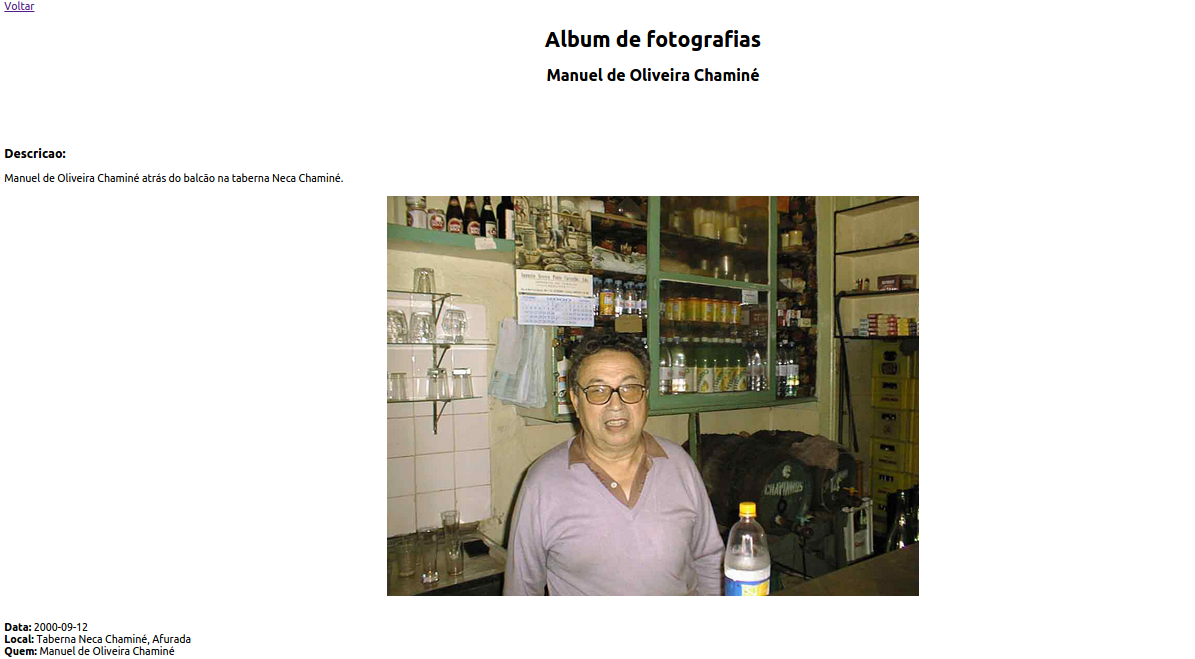
\includegraphics[width=15cm]{anexos/2-1/Exemplo1/Screenshots/pag1.png}
\caption{Pagina HTML gerada pelo ficheiro XML (1 de 2)}
\end{figure}

\begin{figure}[H]
\centering
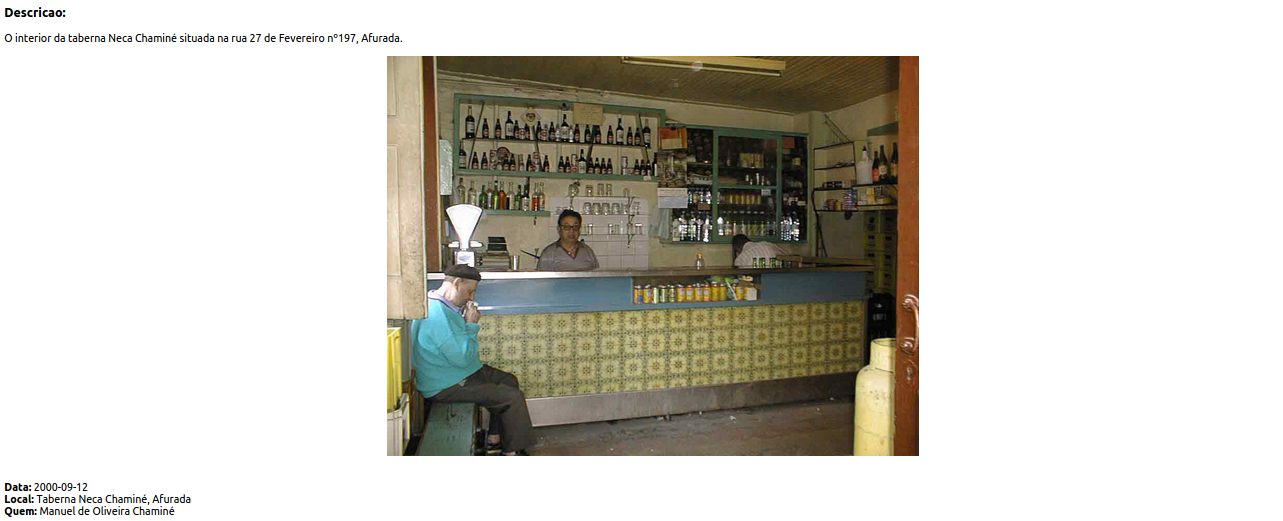
\includegraphics[width=15cm]{anexos/2-1/Exemplo1/Screenshots/pag2.png}
\caption{Pagina HTML gerada pelo ficheiro XML (2 de 2)}
\end{figure}

\subsubsection{Input teste 2}
\label{seq:anex-museu-test-in02}
\lstinputlisting[language=xml]{anexos/2-1/Exemplo2/legenda.xml}

\subsubsection{Output teste 2}
\label{seq:anex-museu-test-out02-01}
\lstinputlisting[language=html]{anexos/2-1/Exemplo2/AlbumGerado.html}

\begin{figure}[H]
\centering

\includegraphics[width=15cm]{anexos/2-1/Exemplo2/Screenshots/indice.png}
\caption{Indice HTML gerado pelo ficheiro XML}
\end{figure}

\label{seq:anex-museu-test-out02-02}
\lstinputlisting[language=html]{anexos/2-1/Exemplo2/5.html}

\begin{figure}[H]
\centering
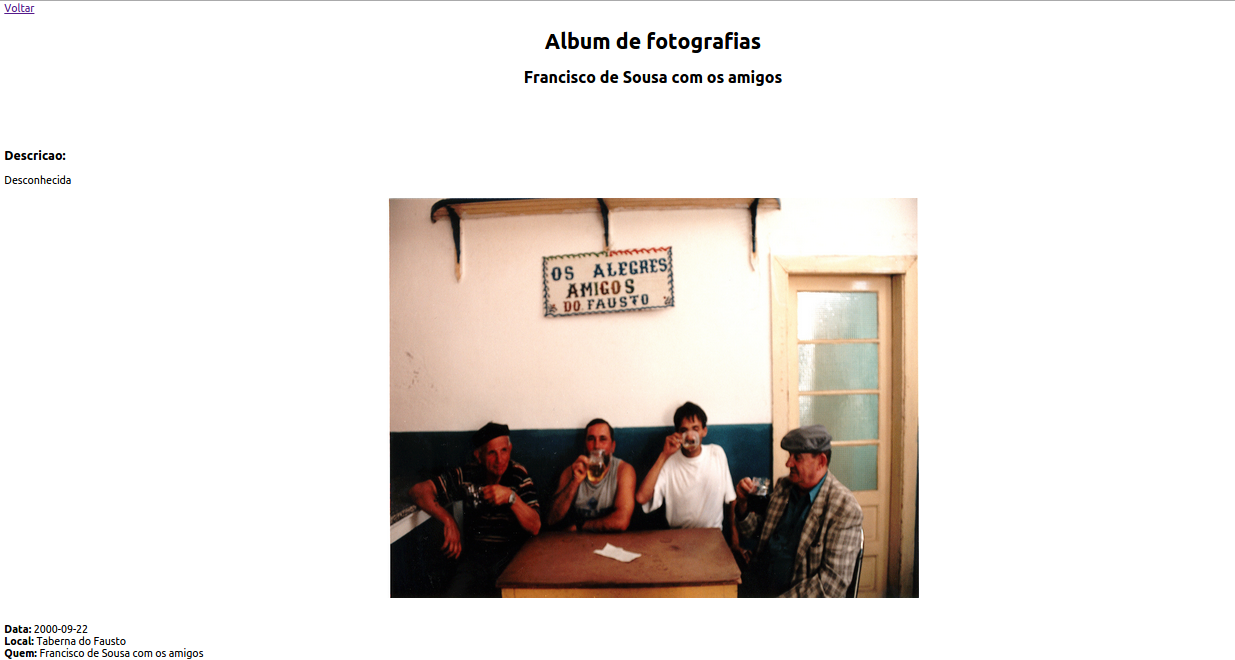
\includegraphics[width=15cm]{anexos/2-1/Exemplo2/Screenshots/pag1.png}
\caption{Pagina HTML gerada pelo ficheiro XML}
\end{figure}

\label{seq:anex-museu-test-out02-03}
\lstinputlisting[language=html]{anexos/2-1/Exemplo2/6.html}

\begin{figure}[H]
\centering
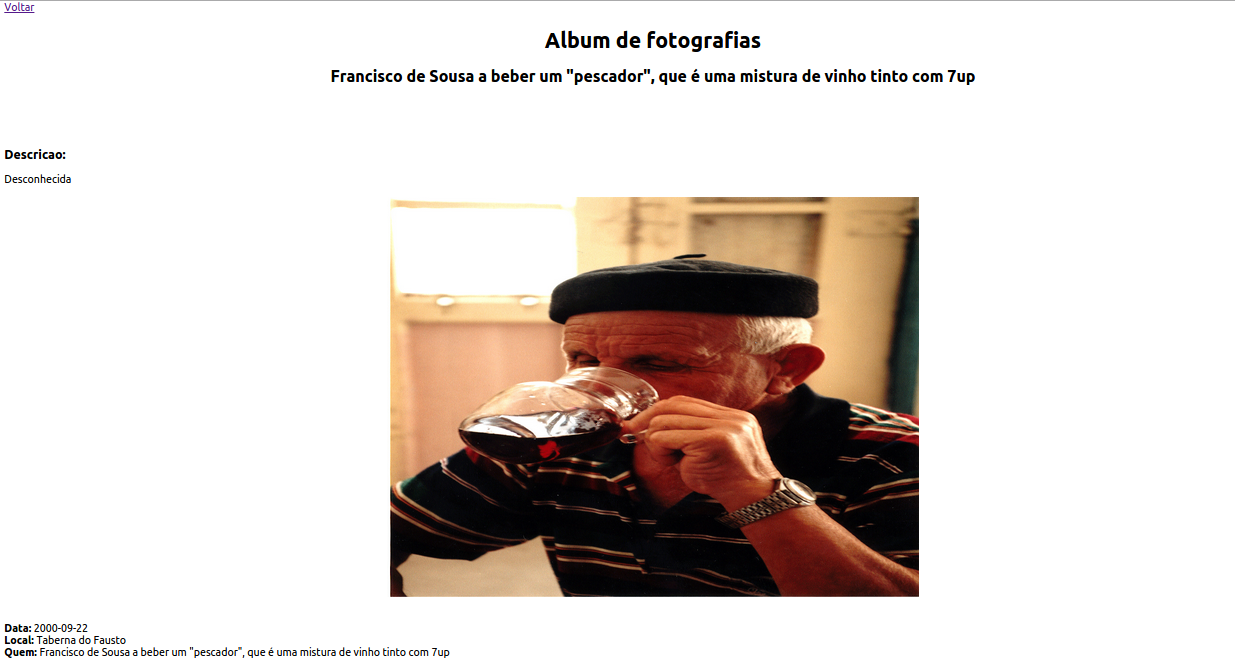
\includegraphics[width=15cm]{anexos/2-1/Exemplo2/Screenshots/pag2.png}
\caption{Pagina HTML gerada pelo ficheiro XML}
\end{figure}

\subsubsection{Input teste 3}
\label{seq:anex-museu-test-in03}
\lstinputlisting[language=xml]{anexos/2-1/Exemplo3/legenda.xml}

\subsubsection{Output teste 3}
\label{seq:anex-museu-test-out03-01}
\lstinputlisting[language=html]{anexos/2-1/Exemplo3/AlbumGerado.html}

\begin{figure}[H]
\centering

\includegraphics[width=15cm]{anexos/2-1/Exemplo3/Screenshots/indice.png}
\caption{Indice HTML gerado pelo ficheiro XML}
\end{figure}

\label{seq:anex-museu-test-out03-02}
\lstinputlisting[language=html]{anexos/2-1/Exemplo3/3.html}

\begin{figure}[H]
\centering
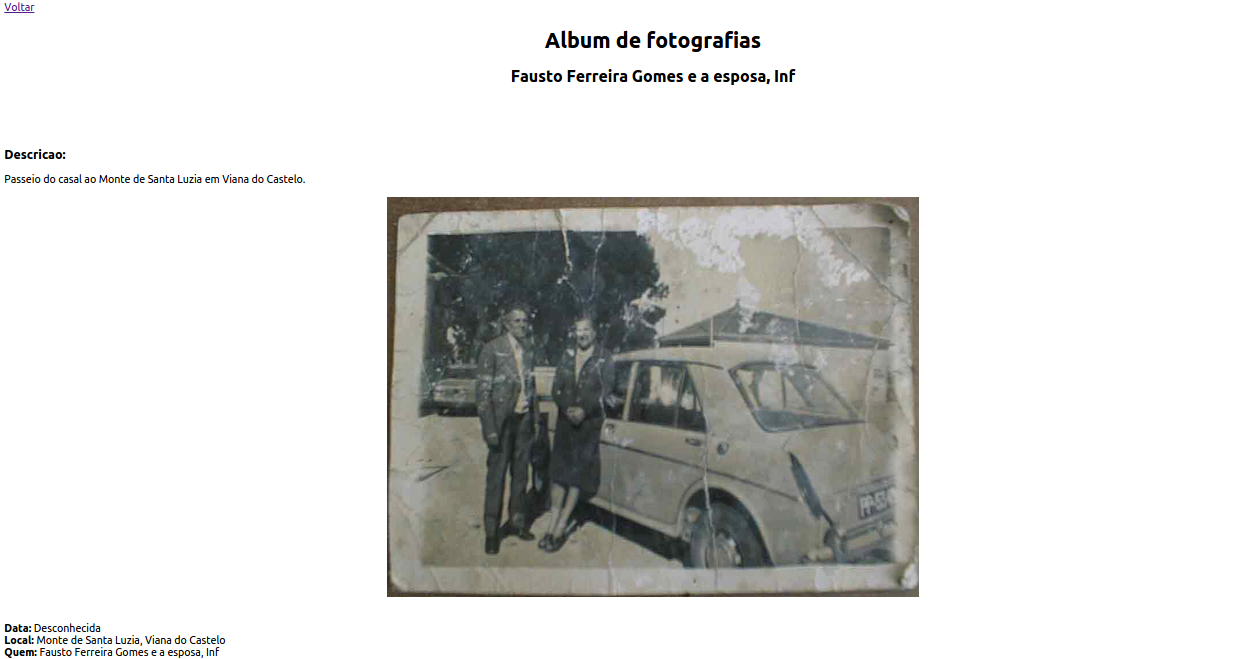
\includegraphics[width=15cm]{anexos/2-1/Exemplo3/Screenshots/pag2.png}
\caption{Pagina HTML gerada pelo ficheiro XML}
\end{figure}

\label{seq:anex-museu-test-out03-03}
\lstinputlisting[language=html]{anexos/2-1/Exemplo3/4.html}

\begin{figure}[H]
\centering
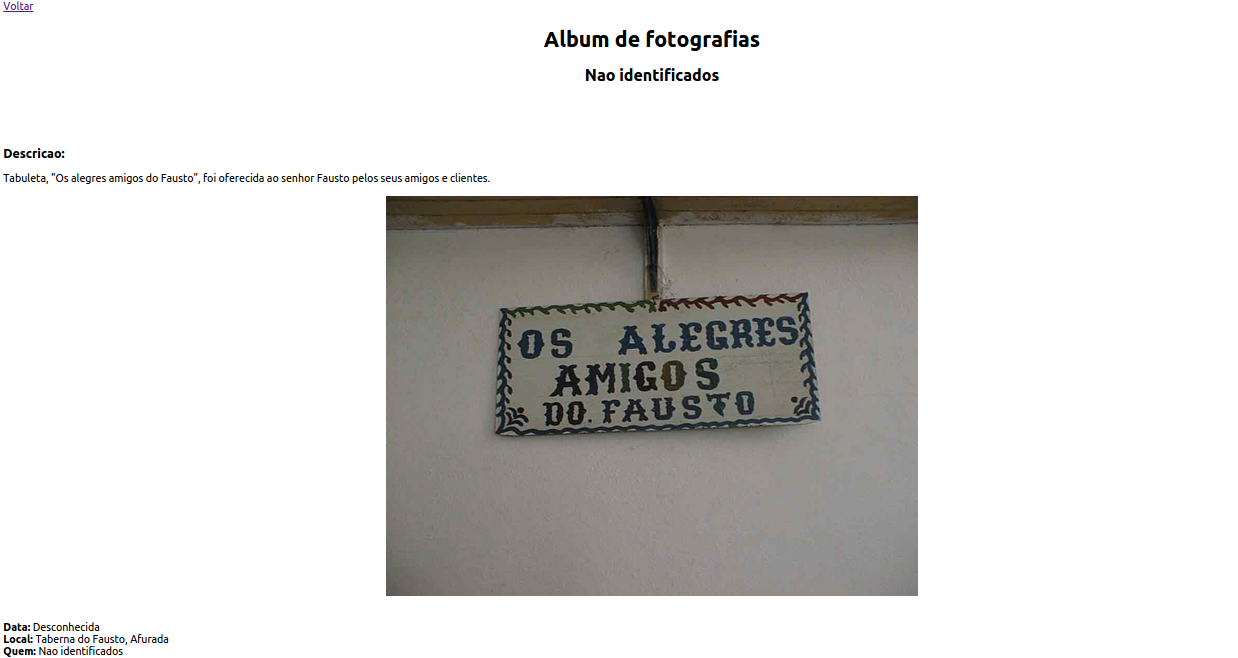
\includegraphics[width=15cm]{anexos/2-1/Exemplo3/Screenshots/pag1.png}
\caption{Pagina HTML gerada pelo ficheiro XML}
\end{figure}

\subsubsection{Input teste 4}
\label{seq:anex-museu-test-in04}
\lstinputlisting[language=xml]{anexos/2-1/Exemplo4/exemplo.xml}

\subsubsection{Output teste 4}
\label{seq:anex-museu-test-out04-01}
\lstinputlisting[language=html]{anexos/2-1/Exemplo4/AlbumGerado.html}

\begin{figure}[H]
\centering

\includegraphics[width=15cm]{anexos/2-1/Exemplo4/Screenshots/indice.png}
\caption{Indice HTML gerado pelo ficheiro XML}
\end{figure}

\label{seq:anex-museu-test-out04-02}
\lstinputlisting[language=html]{anexos/2-1/Exemplo4/1.html}

\begin{figure}[H]
\centering
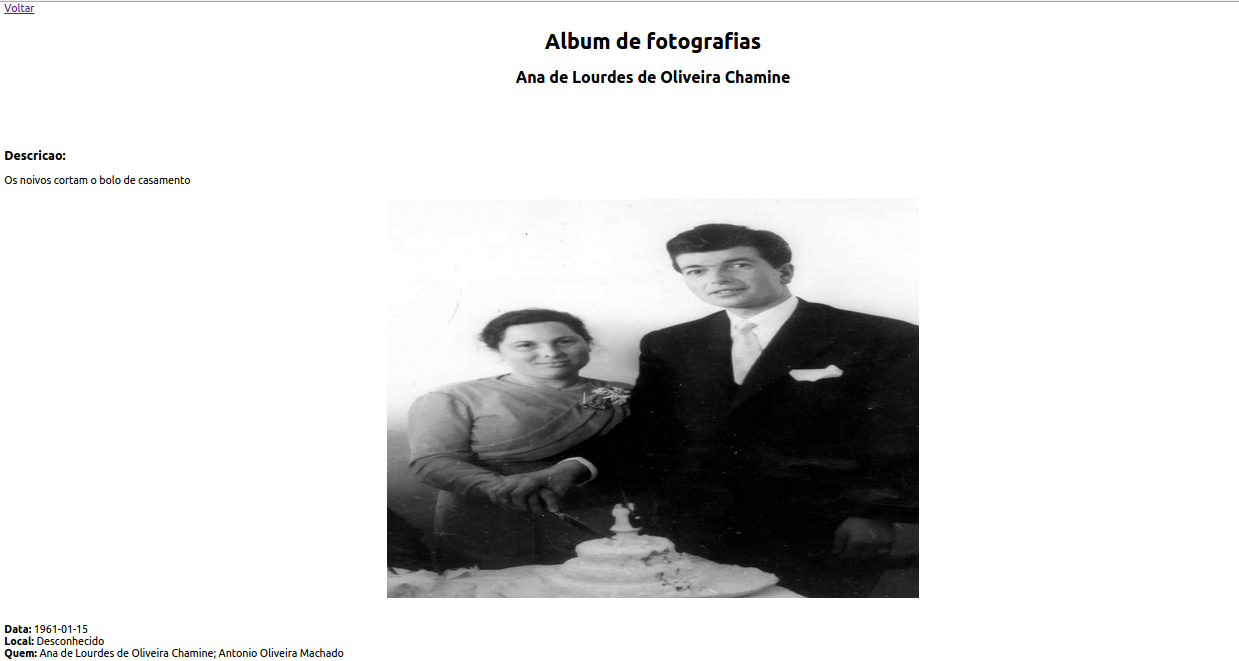
\includegraphics[width=15cm]{anexos/2-1/Exemplo4/Screenshots/pag1.png}
\caption{Pagina HTML gerada pelo ficheiro XML}
\end{figure}

\label{seq:anex-museu-test-out04-03}
\lstinputlisting[language=html]{anexos/2-1/Exemplo4/2.html}

\begin{figure}[H]
\centering
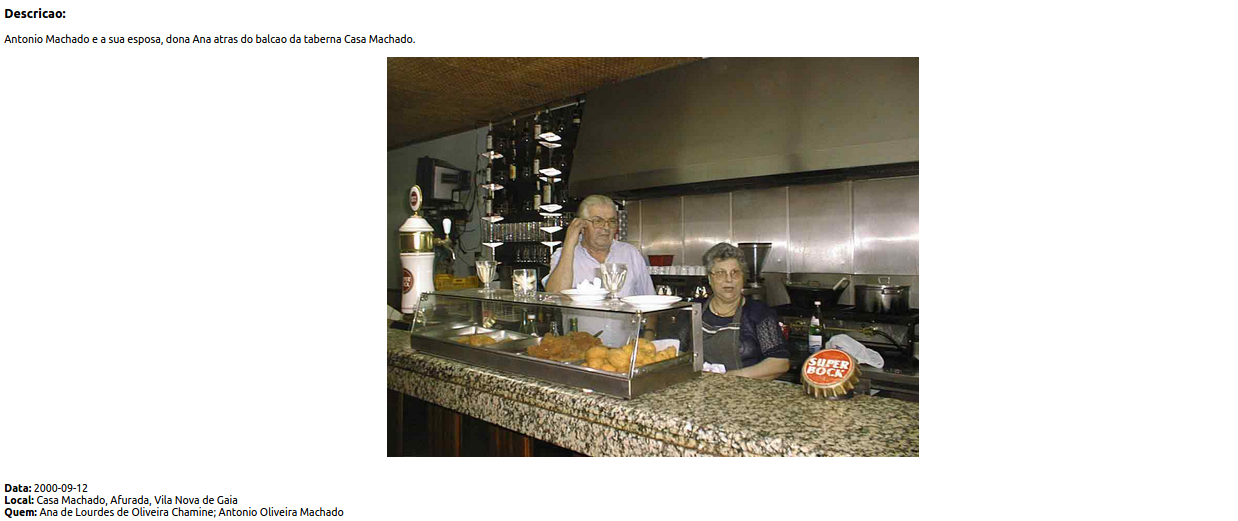
\includegraphics[width=15cm]{anexos/2-1/Exemplo4/Screenshots/pag2_2.png}
\caption{Pagina HTML gerada pelo ficheiro XML}
\end{figure}

\section{Processamento de Entidades Nomeadas (Enamex)}
\label{seq:anex-enamex}

\subsection{Filtro de Texto}
\label{seq:anex-enamex-filtro}
\verbatiminput{anexos/2-2/enamex.l}

\subsection{Estrutura de dados}
\label{seq:anex-enamex-est}
\lstinputlisting[language=c]{anexos/2-2/tree.c}

\subsection{Cabeçalho ficheiro C}
\label{seq:anex-enamex-header}
\lstinputlisting[language=c]{anexos/2-2/tree.h}


\subsection{Testes}
\label{seq:anex-enamex-test}
\subsubsection{Input teste 1}
\label{seq:anex-enamex-test-in01}
\lstinputlisting[language=xml,breaklines=true]{anexos/2-2/teste1_locais.txt}

\subsubsection{Output teste 1}
\label{seq:anex-enamex-test-out01}
\verbatiminput{anexos/2-2/2-5-a-out}
\begin{figure}[H]
\centering
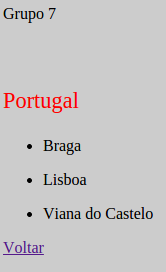
\includegraphics[width=4cm]{anexos/2-2/output_teste1.png}
\end{figure}


\subsubsection{Input teste 2}
\label{seq:anex-enamex-test-in02}
\lstinputlisting[language=xml,breaklines=true]{anexos/2-2/teste2_enunciado.txt}

\subsubsection{Output teste 2}
\label{seq:anex-enamex-test-out02}
\verbatiminput{anexos/2-2/2-5-a-out}
\begin{figure}[H]
\centering
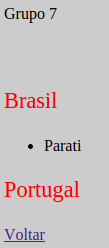
\includegraphics[width=4cm]{anexos/2-2/output_teste2.png}
\end{figure}

\subsubsection{Input teste 3}
\label{seq:anex-enamex-test-in03}
\lstinputlisting[language=xml,breaklines=true]{anexos/2-2/teste3_internet.txt}

\subsubsection{Output teste 3}
\label{seq:anex-enamex-test-out03}
\verbatiminput{anexos/2-2/2-5-a-out}
\begin{figure}[H]
\centering
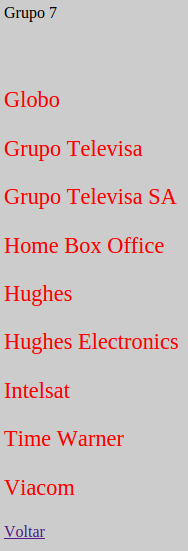
\includegraphics[width=4cm]{anexos/2-2/output_teste3.png}
\end{figure}






\section{Processamento de ficheiros com Canções}
\label{seq:anex-music}

\subsection{Filtro de Texto}
\label{seq:anex-music-filtro}
\verbatiminput{anexos/2-5/flex.l}

\subsection{Estrutura de dados}
\label{seq:anex-music-est}
\lstinputlisting[language=c]{anexos/2-5/musica.c}

\subsection{Cabeçalho ficheiro C}
\label{seq:anex-music-header}
\lstinputlisting[language=c]{anexos/2-5/musica.h}

\subsection{Testes}
\label{seq:anex-music-tests}
\subsubsection{Input teste 1}
\label{seq:anex-music-test-in01}
\verbatiminput{anexos/2-5/2-5-a-in}

\subsubsection{Output teste 1}
\label{seq:anex-music-test-out01}
\verbatiminput{anexos/2-5/2-5-a-out}

\subsubsection{Input teste 2}
\label{seq:anex-music-test-in02}
\verbatiminput{anexos/2-5/2-5-a-in}

\subsubsection{Output teste 2}
\label{seq:anex-music-test-out02}
\verbatiminput{anexos/2-5/2-5-b-out}

\subsubsection{Input teste 3}
\label{seq:anex-music-test-in03}
\verbatiminput{anexos/2-5/2-5-c-in}

\subsubsection{Output teste 3}
\label{seq:anex-music-test-out03}
\verbatiminput{anexos/2-5/2-5-c-out}

\begin{figure}
\centering
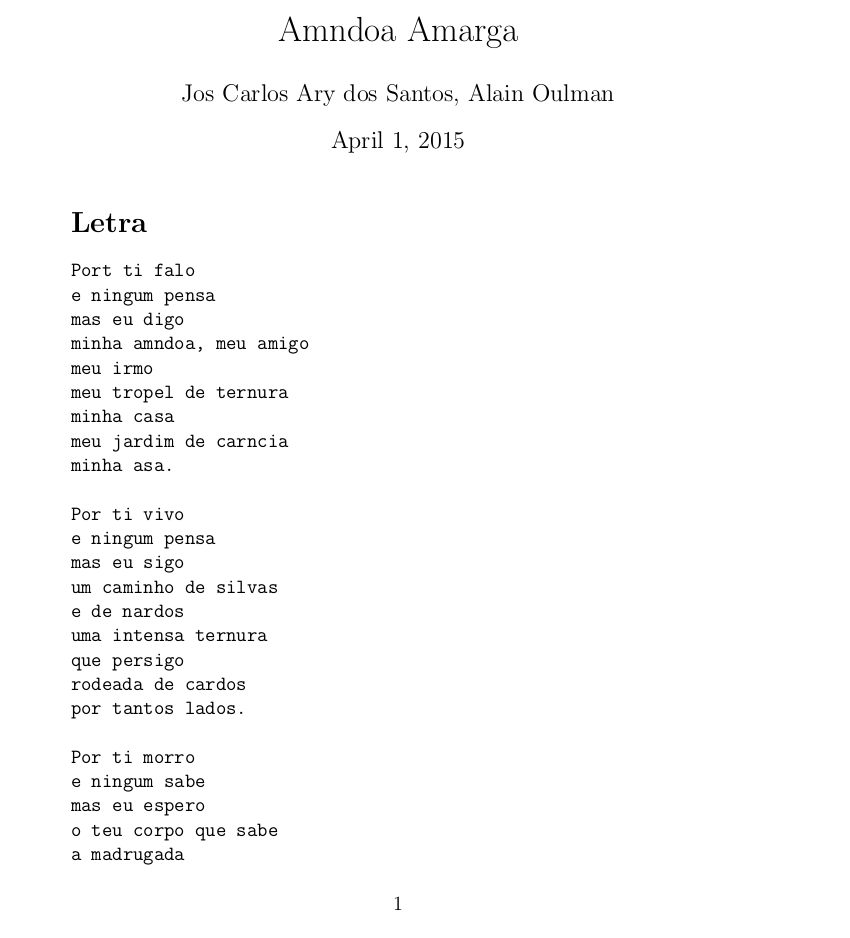
\includegraphics[width=15cm]{anexos/2-5/2-5-a-img1.png}
\caption{PDF gerado por o ficheiro latex (teste 1). Pagina 1 de 2}
\end{figure}

\begin{figure}
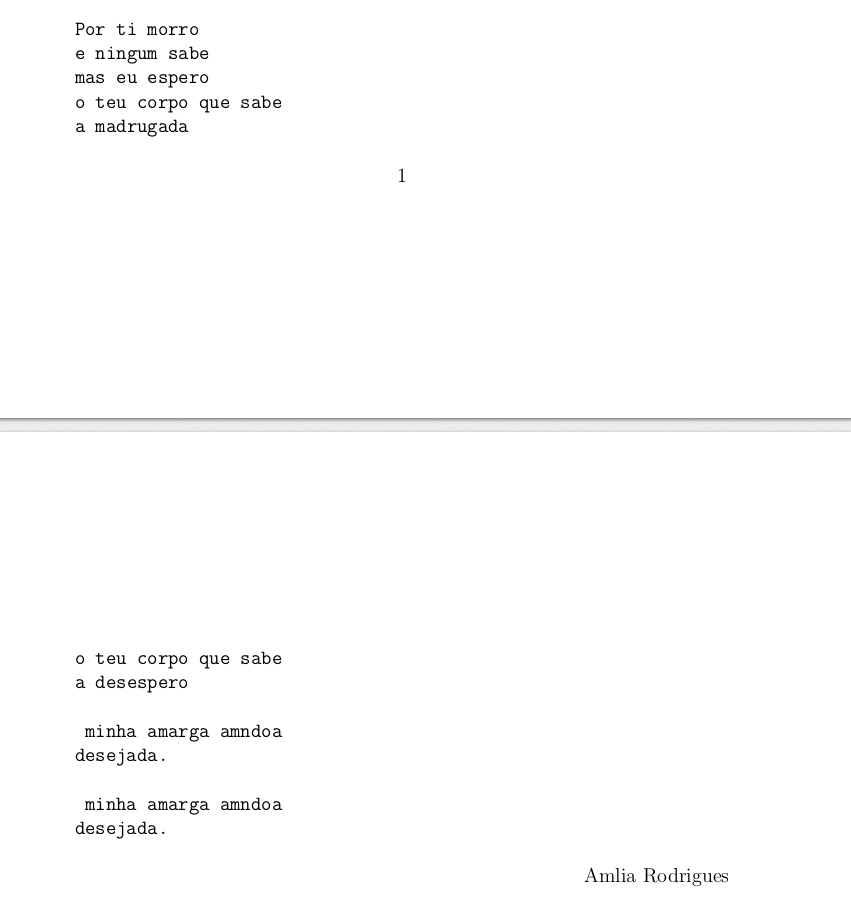
\includegraphics[width=15cm]{anexos/2-5/2-5-a-img2.png}
\caption{PDF gerado por o ficheiro latex (teste 1). Pagina 2 de 2}
\label{fig::anex-music-test-img}
\end{figure}

\begin{figure}
\centering
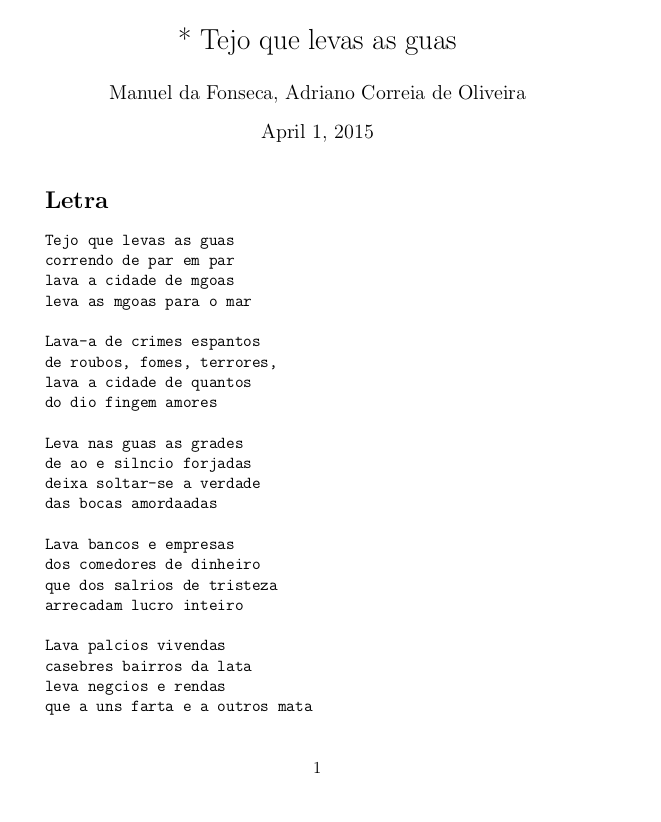
\includegraphics[width=15cm]{anexos/2-5/2-5-b-img.png}
\caption{PDF gerado por o ficheiro latex (teste 2). Pagina 1 de 2}
\label{fig::anex-music-test-img02}
\end{figure}

\begin{figure}
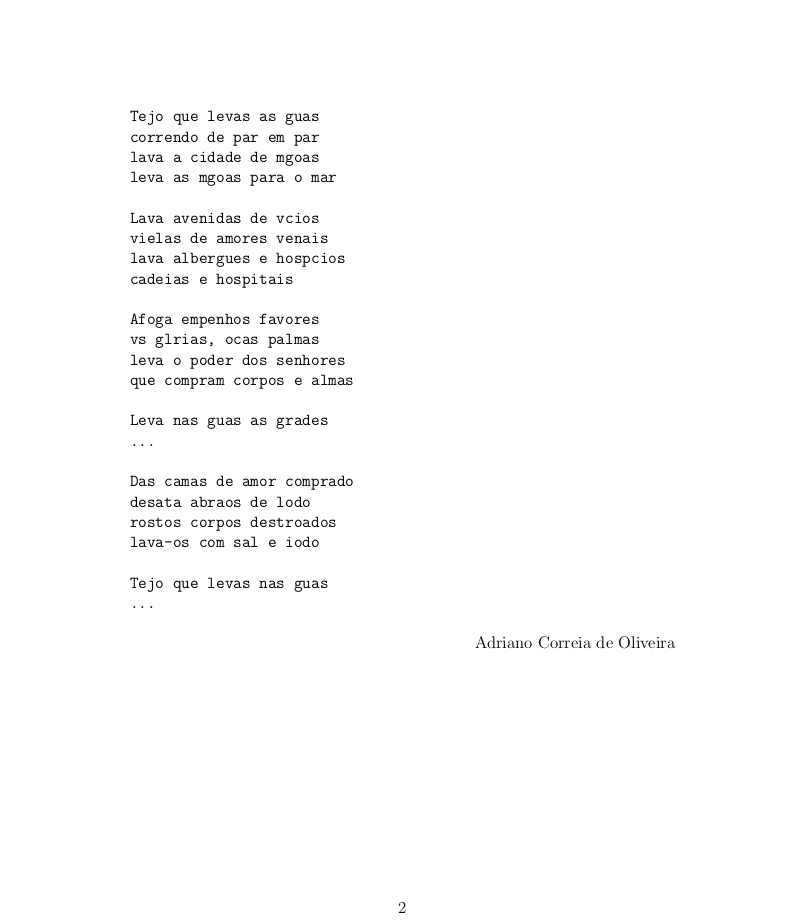
\includegraphics[width=15cm]{anexos/2-5/2-5-b-img2.png}
\caption{PDF gerado por o ficheiro latex (teste 2). Pagina 2 de 2}
\label{fig::anex-music-test-img}
\end{figure}

\begin{figure}
\centering
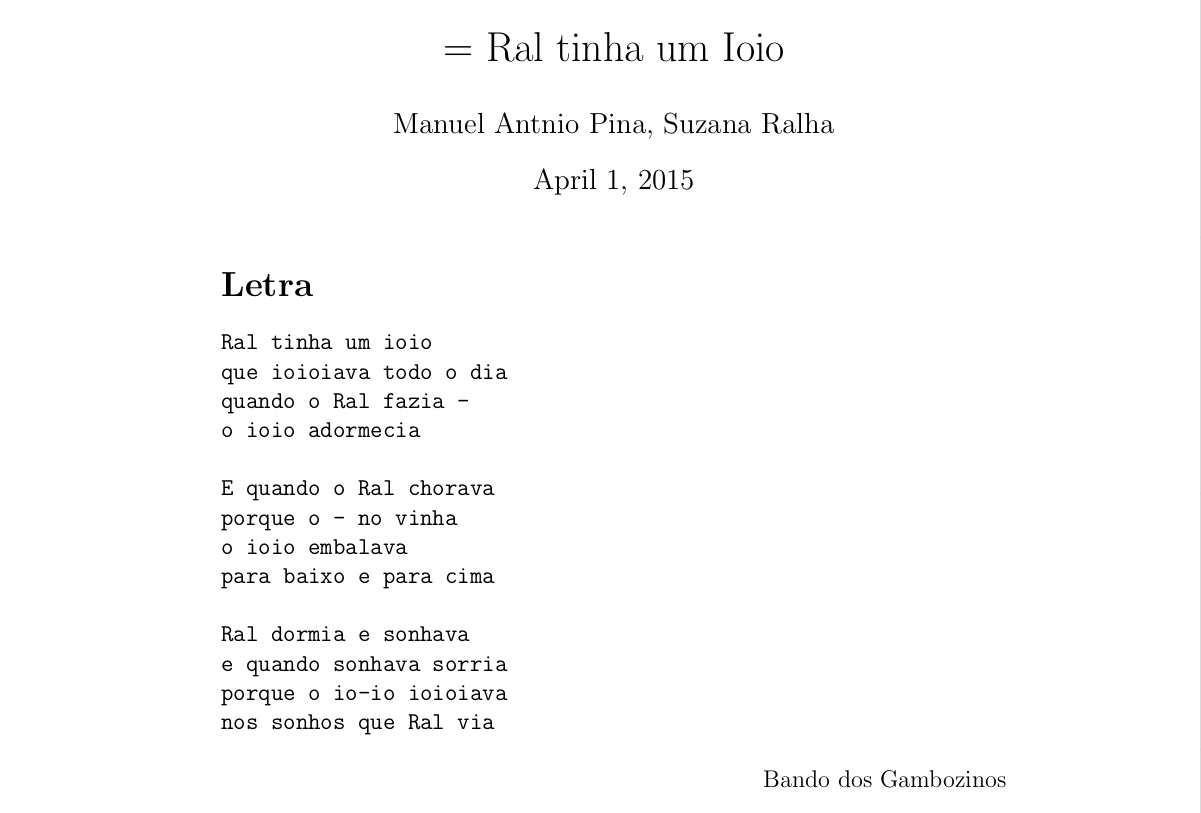
\includegraphics[width=15cm]{anexos/2-5/2-5-c-img.png}
\caption{PDF gerado por o ficheiro latex (teste 3)}
\label{fig::anex-music-test-img03}
\end{figure}
\end{document}


% respectivo enunciado, da descricao do problema, das decisoes que lideraram o desenho da solucao e sua implementacao (incluir a especificacao Flex , deverao conter exemplos de utilizacao (textos fontes diversos e respectivo resultado produzido)